\documentclass{dit}

\usepackage{amsmath}
\usepackage{hyperref}
\pdfstringdefDisableCommands{\def\_{_}}
\usepackage{tikz}
% \usepackage{pgfplots}

% allow embedding files in the PDF so viewers can open/save them
\usepackage{attachfile2}

% CSV import for tables
\usepackage{csvsimple}
\usepackage{longtable}

\usepackage[english,greek]{babel}
% helper to typeset short English fragments when main language is Greek
\newcommand{\en}[1]{\foreignlanguage{english}{#1}}

\newcommand*{\name}{Ευάγγελος Τραϊκόγλου}
\newcommand*{\id}{1115202200189}
\newcommand*{\course}{Παράλληλα Συστήματα}
\newcommand*{\assignment}{Εργασία \en{Pthreads}}

\begin{document}

\maketitle

% \tableofcontents
\begin{itemize}
    \item \en{cpu}: \en{i7-8700}
    \item \en{cores}: \en{12 logical, 6 physical}
    \item \en{os, kernel}: \en{Ubuntu 24.04.3 LTS, 6.8.0-87-generic}
    \item \en{comp version}: \en{gcc 13.3.0}
\end{itemize}

\section{\en{Polynomial Multiplication}}
Η πρώτη άσκηση επικεντρώνεται στον πολλαπλασιασμό πολυωνύμων βαθμού \en{n}.
Ο σειριακός αλγόριθμος ακολουθεί την απλή υλοποίηση $\mathcal{O}(n^2)$ χρόνου.
Στον παράλληλο, κάθε νήμα υπολογίζει ένα εύρος του διανύσματος αποτελέσματος μεγέθους
$\left\lceil (2n+1)/nthreads \right\rceil$, σύμφωνα με τον τύπο: 
$res_k = \sum_{i=0}^{k}a_i \cdot b_{k-i}$. Αυτό επιτρέπει τη μη χρήση συγχρονισμού αφού κάθε νήμα
γράφει σε διαφορετικές θέσεις. Και οι δύο (για βαθμό ή φορτίο $\geq$ 1024) χρησιμοποιούν
εκδοχή με \en{blocking} (\en{bs} = 128), αφού πετυχαίνεται καλύτερη απόδοση από τον βαθμό αυτό και μετά.

% Figures for Polynomial Multiplication
\begin{figure}[htbp]
    \centering
    
\includegraphics[width=0.8\linewidth]{graphs/execution_time_vs_threads_pol.png}
    \caption{\en{Execution time vs threads for polynomial multiplication}}
    \label{fig:exec_time_vs_threads_pol}
\end{figure}

\begin{figure}[htbp]
    \centering
    
\includegraphics[width=0.8\linewidth]{graphs/speedup_vs_threads_pol.png}
    \caption{\en{Speedup vs threads for polynomial multiplication}}
    \label{fig:speedup_vs_threads_po}
\end{figure}

\underline{Συμπεράσματα}:
Για μικρά \en{n} (πχ 100), η αύξηση των νημάτων αυξάνει τον χρόνο εκτέλεσης αφού επηρεάζεται
κυρίως από την ύπαρξή τους. Κάθως όμως το \en{n} αυξάνεται, η αύξηση των νημάτων επιφέρει μείωση
του χρόνου εκτέλεσης. Βέβαια το κέρδος από την εισαγωγή ενός νέου νήματος μειώνεται, ακολουθώντας
τον νόμο της φθίνουσας απόδοσης. Αντίστοιχα, η επιτάχυνση (με βάση το σειριακό) μεγιστοποιείται στον
μέγιστο αριθμό από νήματα και για μεγαλύτερες τιμές του \en{n}.

\section{\en{Update Shared Var}}
Η δεύτερη άσκηση επικεντρώνεται στον πιο αποδοτικό τρόπο ανανέωσης μιας κοινόχρηστης μεταβλητής.
Η υλοποίηση με \en{atomic} εντολές χρησιμοποιεί το όρισμα \en{\_\_ATOMIC\_RELAXED} αφού δε
χρειάζεται κάποια διάταξη όσο αναφορά τις αναφορές στη μνήμη πριν ή μετά την \en{atomic} εντολή.

% UV figures for Update Shared Var
\begin{figure}[htbp]
    \centering
    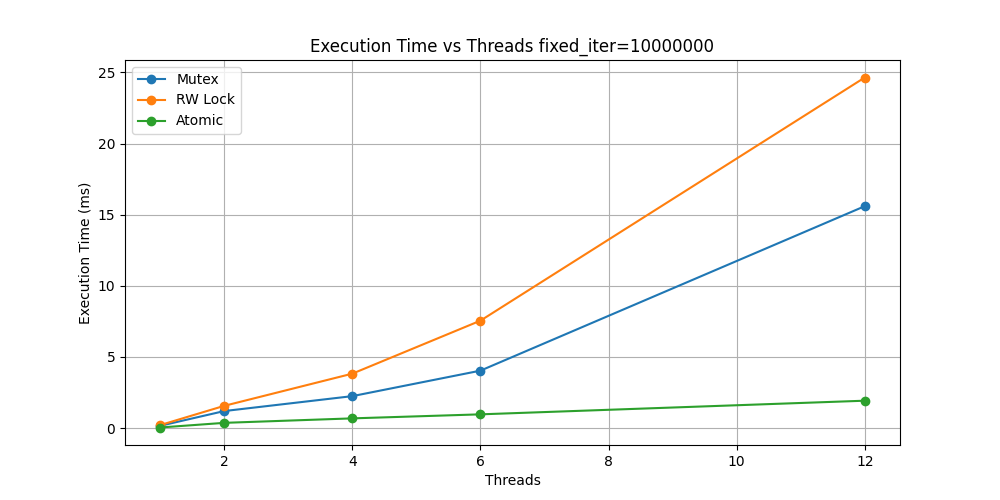
\includegraphics[width=0.8\linewidth]{graphs/time_vs_threads_uv.png}
    \caption{\en{Execution time vs threads (update shared var)}}
    \label{fig:time_vs_threads_uv}
\end{figure}

\begin{figure}[htbp]
    \centering
    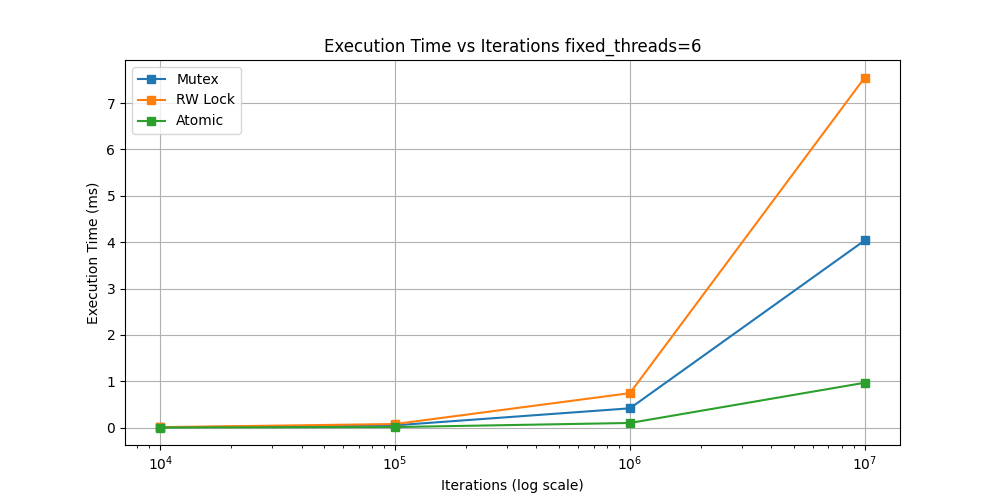
\includegraphics[width=0.8\linewidth]{graphs/time_vs_iterations_uv.png}
    \caption{\en{Execution time vs iterations (update shared var)}}
    \label{fig:time_vs_iterations_uv}
\end{figure}



\newpage

% Raw CSV included as selectable text so it can be highlighted/copied in the PDF
\subsection*{\en{All Runs}}
\begin{otherlanguage}{english}
\lstinputlisting[basicstyle=\ttfamily\small,breaklines=true,columns=fullflexible]{csv/results_uv.csv}
\end{otherlanguage}

\underline{Συμπεράσματα}:
Η υλοποίηση με την \en{atomic} εντολή είναι η πιο γρήγορη για όλα τα πειράματα που έγιναν, μετά
τα \en{mutexes} και τέλος τα \en{rwlocks}. Αυτό είναι λογικό αφού οι \en{atomic} εντολές υποστηρίζονται
από το \en{hardware}. Μεταξύ των \en{mutexes} και \en{rwlocks}, ο επιπρόσθετος χρόνος των 2ων είναι γιατί
έχουν πιο σύνθετη υλοποίηση, λύνοντας το \en{readers-writers} πρόβλημα. Όταν όμως χρησιμοποιούνται σαν \en{mutexes}
(όπως εδώ), επιβαρύνουν τον χρόνο εκτέλεσης.


\section{\en{Table Stats}}
Η τρίτη άσκηση αφορά τη καταμέτρηση των μη μηδενικών στοιχείων 4 πινάκων σε 4 νήματα σε μια κοινή δομή.
Ανάλογα αν έχει οριστεί η \en{IMPROVED} χρησιμοποιείται ή όχι η βελτιωμένη εκδοχή, όπου το \en{struct} είναι
\en{padded} για να γεμίζει ένα \en{cache line} ο κάθε μετρητής, για να αποφευχθεί το φαινόμενο του \en{false sharing}.

\begin{figure}[htbp]
    \centering
    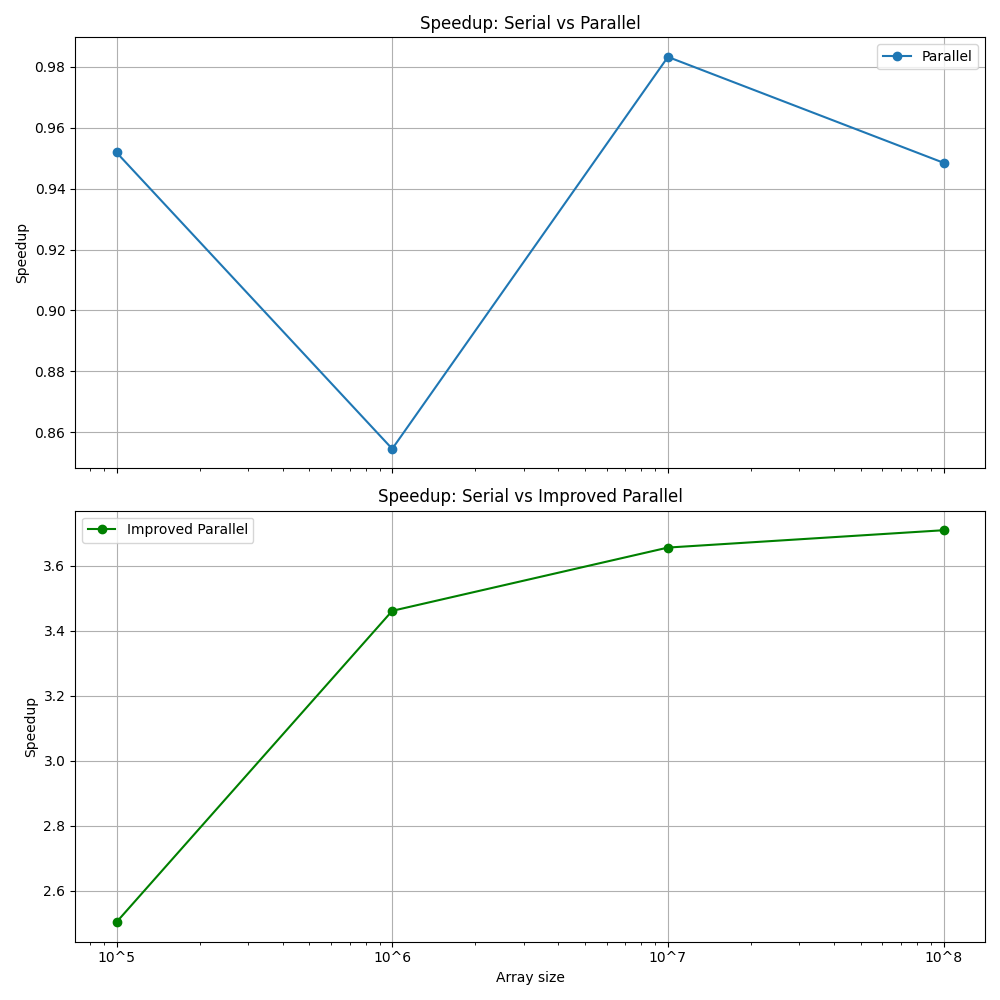
\includegraphics[width=0.8\linewidth]{graphs/serial_vs_par.png}
    \caption{\en{Speedup: Serial vs Parallel}}
    \label{fig:time_vs_threads_uv}
\end{figure}

\begin{figure}[htbp]
    \centering
    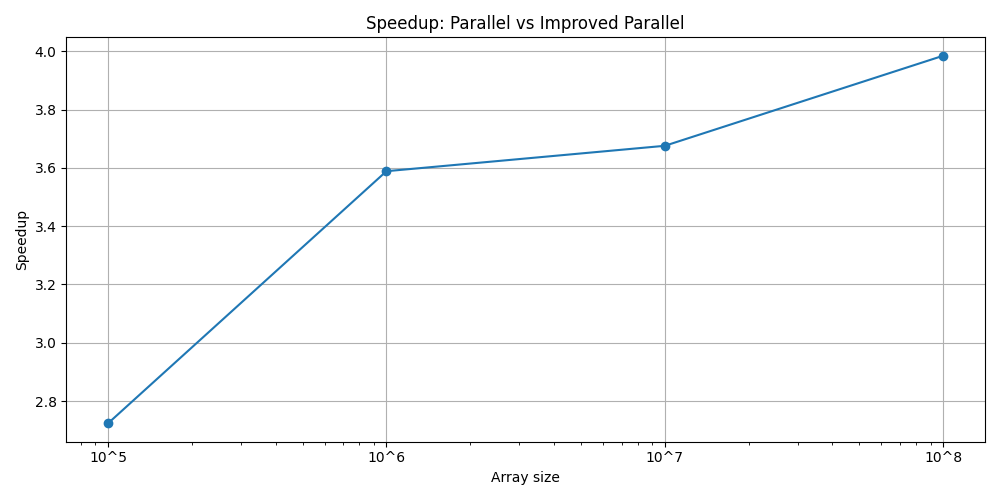
\includegraphics[width=0.8\linewidth]{graphs/speedup_parallel_vs_improved.png}
    \caption{\en{Speedup: Parallel vs improved}}
    \label{fig:time_vs_iterations_uv}
\end{figure}

\underline{Συμπεράσματα}:
Αρχικά, δεν χρειάζεται συγχρονισμός αφού κάθε νήμα γράφει σε διαφορετική μεταβλητή.
Ο απερίσκεπτος παράλληλος αλγόριθμος δεν επιτυγχάνει καμία βελτίωση έναντι του σειριακού.
Αυτό δείχνει πόσο το \en{false sharing} επηρεάζει την απόδοση. Η βελτιωμένη εκδοχή όπου
το κάθε \en{cache line} έχει έναν μετρητή πλησιάζει την ιδανική επιτάχυνση (\en{x4}) καθώς το
\en{n} αυξάνεται.

\newpage

\section{\en{Bank}}
Η τέταρτη άσκηση προσομοιώνει τη λειτουργία μιας τράπεζας. Κάθε νήμα κάνει ένα μείγμα συναλλαγών
(μεταφοράς χρημάτων, ερώτησης υπολοίπου). Χρησιμοποιούνται δύο είδη κλειδομάτων (\en{mutexes,rwlocks}).
Το ζητούμενο είναι να μελετηθεί η επίδραση της επιλογής των κλειδωμάτων στις διάφορες επιλογές παραμέτρων.
Υλοποιήθηκαν \en{wrapper functions lock,unlock} (Προφανώς η επιλογή \en{READ,WRITE} στη \en{lock} έχει νόημα
μόνο για τη περίπτωση των \en{rwlocks}).
\\
\en{thread\_work}: Δύο επιλογές: \en{fine grain: 1 lock} ανά λογαριασμό, \en{coarse grain: 1 lock} για τον πίνακα.
Κάθε νήμα κάνει \en{perc}\% ερωτήσεις υπολοίπου και \en{1-perc}\% μεταφορές χρημάτων. Προφανώς στις μεταφορές πρέπει
να ελέγχεται αν αυτός που στέλνει έχει υπόλοιπο $\geq$ 0. Το μόνο \en{write lock} που χρειάζεται είναι στην ανανέωση
του υπολοίπου του παραλήπτη.

\begin{center}
    \noindent\fbox{%
        \parbox{0.9\linewidth}{\centering
                \textbf{\en{Benchmark file:}} \en{csv/bank\_results.csv}\\[6pt]
        }
    }
\end{center}

% optional inline preview of first lines:
\begin{otherlanguage}{english}
\lstinputlisting[firstline=1,lastline=13,basicstyle=\ttfamily\small,breaklines=true,columns=fullflexible]{csv/bank_results.csv}
\end{otherlanguage}

% first part
\underline{Συμπεράσματα}:


\newpage

\subsection*{\en{CS = 100 microseconds}}
\begin{otherlanguage}{english}
\lstinputlisting[basicstyle=\ttfamily\small,breaklines=true,columns=fullflexible]{csv/bank_results_sleep.csv}
\end{otherlanguage}

% second part
\underline{Συμπεράσματα}:


\section{\en{Barrier}}

\underline{Συμπεράσματα}:
\end{document}